\lecture{Základní principy \hologo{LaTeX}u}{lec:BasicPrinciples}

\subsection{Co je \hologo{LaTeX}}
\begin{frame}
	\frametitle{Co je \hologo{LaTeX}}
	\begin{itemize}
		\item \hologo{LaTeX} (v češtině vyslovujeme jako \enquote{latech}) je nástroj pro přípravu profesionálně vyhlížejících dokumentů (\emph{document preparation system}).
		\item \hologo{LaTeX} je založen na \emph{WYSIWYM} (What You See Is What You Mean) přístupu -- autor se soustředí na obsah dokumentu, sazeč a počítač se starají o vzhled dokumentu.
	\end{itemize}
	\begin{example}
		Bakalářská práce -- Vy píšete text práce, kreslíte schémata, sestavujete tabulky. Na FEI existuje \enquote{šablona} pro \hologo{LaTeX}, kterou sestavil \enquote{sazeč}, který stanovil rozměry textu, písmo, vzhled nadpisů, pořadí stránek a tak dále.
	\end{example}
\end{frame}


{
	\usebackgroundtemplate
	{
		\begin{tikzpicture}[remember picture, overlay]
			\node at (current page.center) {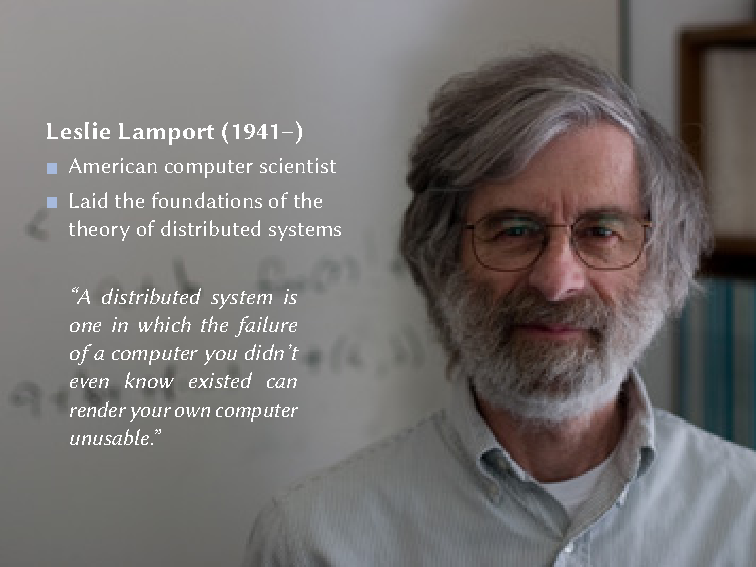
\includegraphics[width=\paperwidth, height=\paperheight, keepaspectratio]{Lecture1/Figures/LL.pdf}};
		\end{tikzpicture}
	}
	\begin{frame}
	\end{frame}
}


\begin{frame}
	\frametitle{Co je \hologo{TeX}}
	\begin{itemize}
		\item \hologo{TeX} je program pro počítačovou sazbu (\emph{computer typesetting system}).
		\item \hologo{TeX} vyslovujeme jako \enquote{tech}. Tři písmena v názvu jsou řecká \enquote{tau-epsilon-chí}. Odvozeno od řeckého \texttau\textepsilon\textchi\textnu\texteta{} [techné], \enquote{umění}, \enquote{dovednost}.
		\item První verze \hologo{TeX}u pochází roku 1978, aktuální 3.14159265 z~března 2014.
		\item Zatímco \hologo{LaTeX} je formát dokumentu, \emph{značkovací jazyk}, \hologo{TeX} je \emph{kompilátor}, který překládá zdrojové kódy zapsané v \hologo{LaTeX}u do cílového jazyka, například Pdf.
	\end{itemize}
\end{frame}


{
	\usebackgroundtemplate
	{
		\begin{tikzpicture}[remember picture, overlay]
			\node at (current page.center) {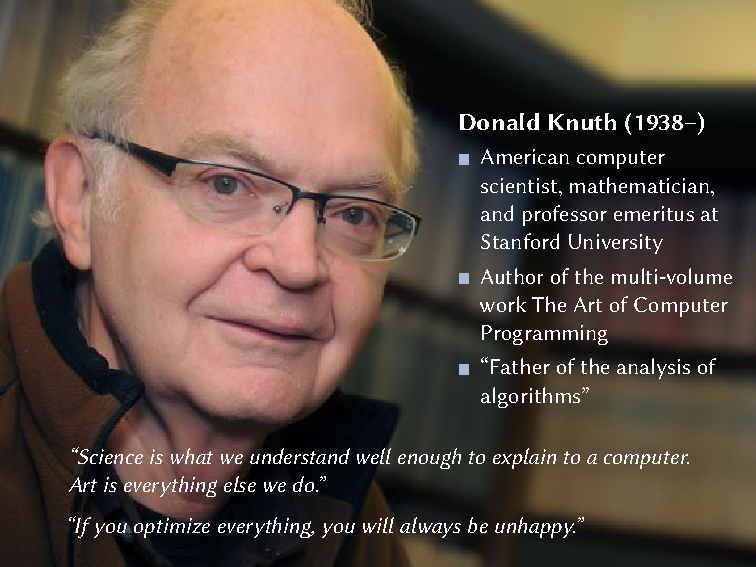
\includegraphics[width=\paperwidth, height=\paperheight, keepaspectratio]{Lecture1/Figures/DEK.pdf}};
		\end{tikzpicture}
	}
	\begin{frame}
	\end{frame}
}


\begin{frame}
	\frametitle{\hologo{TeX}, \hologo{LaTeX} a okolí}
	\begin{description}
		\item[\hologo{LaTeX}] -- značkovací jazyk (obdoba: jazyk HTML)
		\item[\hologo{TeX}] -- překladač (obdoba: renderovací jádro, lze jich mít víc)
		\item[\hologo{pdfTeX}] -- překladač s přímým výstupem do Pdf,
		\item[\hologo{pdfLaTeX}] -- překladač jazyka \hologo{LaTeX}, postavený nad \hologo{pdfTeX}em
		\item[další překladače]\mbox{}
			\begin{itemize}
				\item \hologo{XeTeX} -- nativní podpora UTF-8, přístup k~systémovým fontům,
				\item \hologo{LuaTeX} -- integrace skriptovacího jazyka Lua.
			\end{itemize}
		\item[další programy]\mbox{}
			\begin{itemize}
				\item \hologo{biber}, \hologo{BibTeX} -- zpracování bibliografie,
				\item MakeIndex, xindy -- zpracování rejstříků.
			\end{itemize}
	\end{description}
\end{frame}


\subsection{Proč se učit \hologo{LaTeX}}
\begin{frame}
	\frametitle{Proč se učit \hologo{LaTeX}}
	\begin{columns}[t]
		\begin{column}{0.45\textwidth}
			\begin{block}{Kvalita výstupu}
				\begin{itemize}
					\item sofistikované algoritmy sazby
					\item odvozeno od tradiční typografie
				\end{itemize}
			\end{block}
			\begin{block}{Popularita}
				\begin{itemize}
					\item de-facto norma v~akademickém a~vědeckém světě
				\end{itemize}
			\end{block}
		\end{column}
		\begin{column}{0.48\textwidth}
			\begin{block}{Kvalita software}
				\begin{itemize}
					\item stabilita
					\item rychlost
					\item rozšiřitelnost
					\item vstupním formátem text
					\item mnoho druhů výstupu
				\end{itemize}
			\end{block}
			\begin{block}{Svoboda}
				\begin{itemize}
					\item svobodný software
					\item běží na mnoha platformách
				\end{itemize}
			\end{block}
		\end{column}
	\end{columns}
\end{frame}


\begin{frame}
	\frametitle{Proč se učit \hologo{LaTeX} -- škálovatelnost}
	\begin{center}
		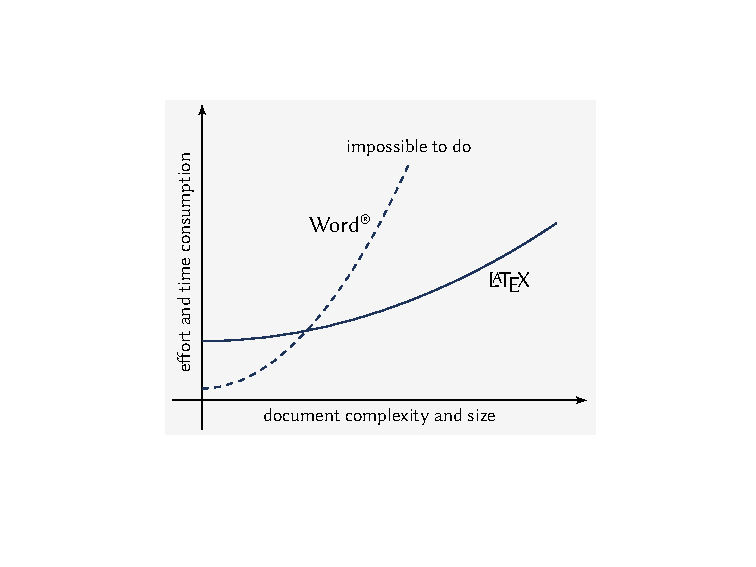
\includegraphics{Lecture1/Figures/Scalability.pdf}\par
		\begin{tiny}
			Převzato z \url{http://www.pinteric.com/miktex.html}
		\end{tiny}
	\end{center}
\end{frame}


\begin{frame}[t]
	\frametitle{Proč se učit \hologo{LaTeX} -- kvalita výstupu}
	\begin{itemize}
		\item Kvalitní sazba a čitelnost
			\begin{itemize}
				\item správné mezery mezi slovy, řádky i odstavci,
				\item kontextově závislé dělení slov,
				\item podpora podřezávání a ligatur.
			\end{itemize}
			\medskip
			\begin{columns}[t]
				\begin{column}{0.45\textwidth}
					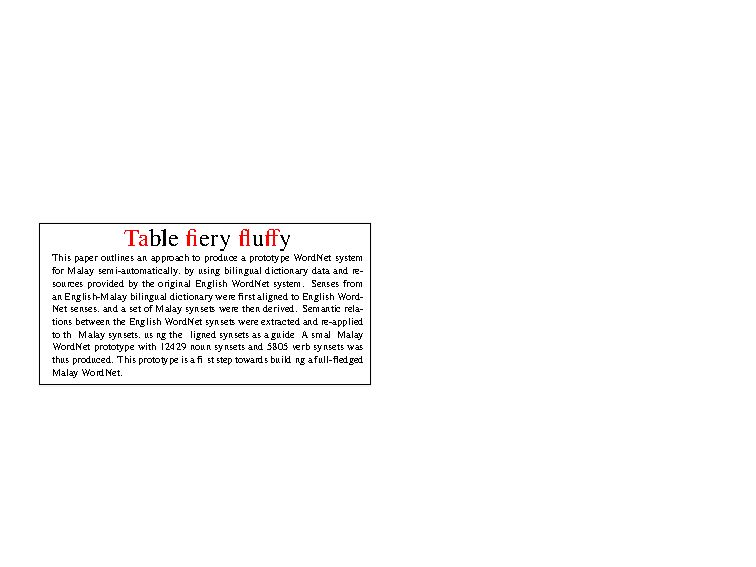
\includegraphics[width=\columnwidth]{Lecture1/Figures/ParagraphSample1.pdf}
				\end{column}
				\begin{column}{0.45\textwidth}
					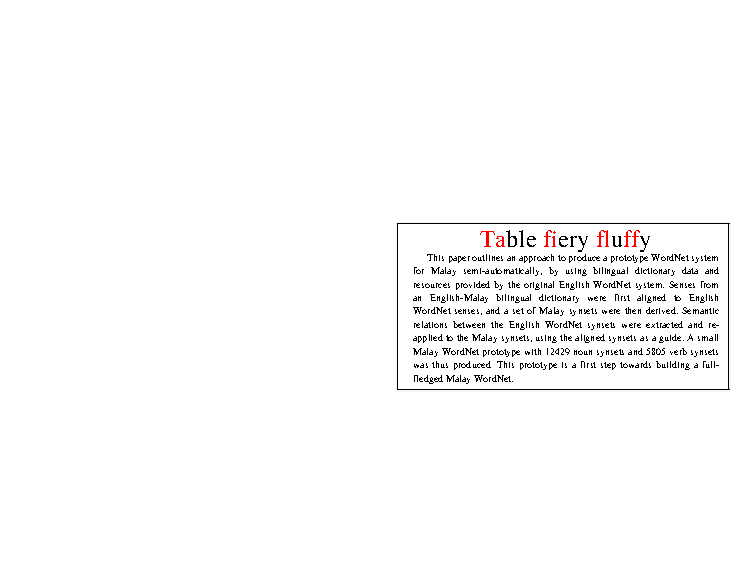
\includegraphics[width=\columnwidth]{Lecture1/Figures/ParagraphSample2.pdf}
				\end{column}
			\end{columns}
		\item Správná matematická sazba
			\begin{columns}[t]
				\begin{column}{0.45\textwidth}
					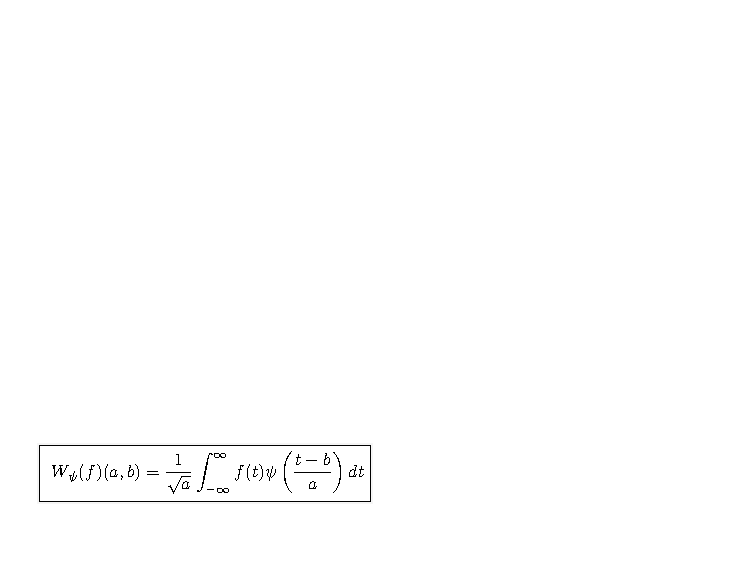
\includegraphics[width=\columnwidth]{Lecture1/Figures/EquationSample1.pdf}
				\end{column}
				\begin{column}{0.45\textwidth}
					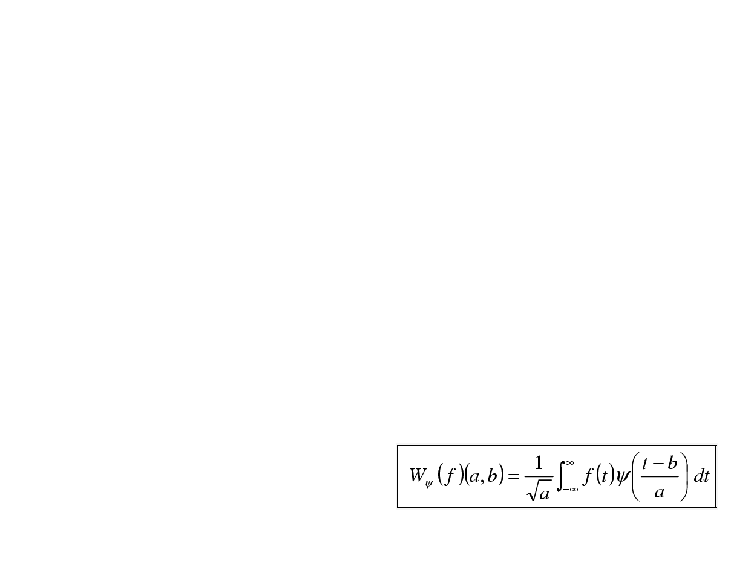
\includegraphics[width=\columnwidth]{Lecture1/Figures/EquationSample2.pdf}
				\end{column}
			\end{columns}
	\end{itemize}
	\begin{center}
		\tiny
		Převzato z \url{http://liantze.penguinattack.org/}.
	\end{center}
\end{frame}


\begin{frame}
	\frametitle{Proč se učit \hologo{LaTeX} -- bakalářská práce}
	\begin{itemize}
		\item Jak jsem posledně formátoval nadpis kapitoly?
		\item Nedával jsem tenhle druh nadpisu kurzívou?
		\item Rovnice se nezobrazuje správně. Někde ano, někde ne!
		\item Do háje, zapomněl jsem aktualizovat obsah dokumentu, nadpisy ani stránky nesedí!
		\item Potřebuji vložit nový obrázek. Jak mám přečíslovat dvacet obrázků?!
		\item Formátování citací a literatury není konzistentní. Jsou pokaždé jiné!
		\item Číslování citací a literatury si neodpovídají!
		\item Editor spadl! \alert{\textbf{Soubor s dokumentem je poškozen! Do pi\ldots!!}} A~zálohu nemám.
	\end{itemize}
\end{frame}


\begin{frame}
	\frametitle{Proč se učit \hologo{LaTeX} -- známé postupy a nástroje}
	\begin{center}
		\emph{Nástroje a postupy používané pro sazbu dokumentů pomocí \hologo{LaTeX}u (\hologo{TeX}u) jsou shodné s~nástroji a postupy používanými pro vývoj software.}
	\end{center}
	\emph{Důležité} -- zdrojový kód dokumentu, obrázky k vložení, konfigurační soubory, atd.\par
	\emph{Nedůležité} -- výsledná podoba dokumentu, vznikne kdykoliv kompilací.\par
	\emph{Známé nástroje a postupy práce} -- dokument jako projekt, správa verzí (Git, Subversion,\ldots), programátorské editory (zvýraznění syntaxe, více otevřených souborů, čistý text), build systémy (např.\ \texttt{make}) nebo integrované vývojové prostředí (IDE).
\end{frame}


\subsection{\hologo{TeX} versus \hologo{LaTeX}}
\begin{frame}
	\frametitle{\hologo{TeX} versus \hologo{LaTeX}}
	\enquote{\emph{Dokument jsem napsal v čistém \hologo{TeX}u.}}
	\begin{itemize}
		\item Virgin \hologo{TeX} -- instrukce sázecího procesoru, \enquote{elementární částice \hologo{TeX}ového vesmíru}, \enquote{nuly a jedničky}.
		\item Čistým \hologo{TeX}em je obvykle míněn formát \hologo{plainTeX}.
		\item \hologo{plainTeX} -- \enquote{assembler}, maximální kontrola nad sazbou dokumentu, ale nutné obrovské předchozí znalosti.
		\item \hologo{LaTeX} -- \enquote{vyšší programovací jazyk}, snadný zápis za cenu jistých omezení (z pohledu \hologo{plainTeX} guru).
		\item Chci \enquote{snadno} napsat technický dokument nebo se \enquote{několik let} učit zvládnout nástroj, kterým dokument psát?
		\item Krásná záminka k tzv.\ flame war.
	\end{itemize}
\end{frame}


\subsection{První dokument v \hologo{LaTeX}u}
\begin{frame}
	\frametitle{První dokument v \hologo{LaTeX}u}
	\begin{enumerate}
		\item V textovém editoru vytvoříme soubor \texttt{FirstDoc.tex} s~následujícím obsahem:\par
			\BVerbatimInput{Samples/FirstDocToInclude.tex}
		\item Na příkazovém řádku spustíme překlad pomocí\\\texttt{pdflatex FirstDoc.tex}
		\item Překladem získáme soubor \texttt{FirstDoc.pdf}
	\end{enumerate}
		\SamplePdfBox{\includegraphics[width=\MaxPdfSampleWidth]{Samples/FirstDoc-crop.pdf}}
\end{frame}


\begin{frame}[fragile]
	\frametitle{První dokument v \hologo{LaTeX}u -- rozbor}
	\BVerbatimInput{Samples/FirstDocToInclude.tex}
	\begin{itemize}
		\item Příkaz |\documentclass| deklaruje \emph{třídu dokumentu}. 
		\item \emph{Preambule} dokumentu
			\begin{itemize}
 				\item oblast mezi |\documentclass| a |\begin{document}|, 
 				\item nastavení parametrů, definice příkazů atd.,
 				\item tato část nesmí generovat viditelný výstup.
			\end{itemize}
		\item Vlastní text dokumentu -- ohraničen |\begin{document}| a~|\end{document}|
	\end{itemize}
\end{frame}


\begin{frame}[fragile]
	\frametitle{První dokument v \hologo{LaTeX}u -- text dokumentu}
	\begin{BVerbatim}
Your first document. This is a very simple example,
with no extra parameters or packages     included.
	\end{BVerbatim}
	\begin{itemize}
		\item Pokud neřekneme jinak, sází \hologo{LaTeX} \emph{odstavce hladkého textu} -- ASCII vstup, zarovnání do bloku, odstavcová zarážka, anglické dělení slov.
		\item Transformace -- konec řádku je nahrazen mezerou, posloupnost mezer je nahrazena jednou mezerou.
		\item Odstavce jsou odděleny aspoň jedním volným řádkem.
	\end{itemize}
	\begin{remark}
		Text dokumentu zapsaný pomocí \hologo{LaTeX}u je zdrojový kód jako každý jiný! Platí jeho úpravu platí obdobná pravidla jako pro každý jiný zdrojový kód, třeba v C++.
	\end{remark}
\end{frame}


\subsection{Distribuce \hologo{TeX}u/\hologo{LaTeX}u}
\begin{frame}[fragile]
	\frametitle{Offline distribuce \hologo{TeX}u/\hologo{LaTeX}u}
	\begin{itemize}
		\item Podobně jako OS Linux, je \hologo{LaTeX} a podpůrný software dostupný ve formě tzv.\ \emph{distribucí}.
		\item Offline distribuce jsou určeny pro lokální instalaci.
	\end{itemize}
	\begin{description}
		\item[\hologo{TeX}Live] -- \url{https://www.tug.org/texlive/}
		\item[Mik\hologo{TeX}] -- \url{https://miktex.org/}
		\item[Mac\hologo{TeX}] -- \url{https://tug.org/mactex/}
	\end{description}
	\begin{block}{Podpora operačních systémů}
		\centering
		\UndefineShortVerb{\|}
		\begin{tabular}{lccc}
			& Windows & Linux & Mac OS\\
			\hline
			\hologo{TeX}Live & \Checkmark & \Checkmark & \XSolidBrush \\
			Mik\hologo{TeX} & \Checkmark & \XSolidBrush & \XSolidBrush \\
			Mac\hologo{TeX} & \XSolidBrush & \XSolidBrush & \Checkmark \\
		\end{tabular}
	\end{block}
\end{frame}


\begin{frame}[fragile]
	\frametitle{Online distribuce \hologo{LaTeX}u}
	\begin{center}
		
\includegraphics[width=0.5\textwidth]{Lecture1/Figures/overleaf_wide_colour_light_bg.pdf}\\
		\url{https://www.overleaf.com/}
	\end{center}
	\begin{itemize}
		\item pro práci je potřebný jen webový prohlížeč a připojení k~internetu,
		\item dokumenty jsou uloženy na serveru Overleaf.com,
		\item snadné sdílení dokumentů,
		\item kolaborativní editace dokumentů,
		\item sledování změn v dokumentu,
		\item integrovaný realtime prohlížeč dokumentů.
	\end{itemize}
\end{frame}


\begin{frame}
	\frametitle{Online distribuce \hologo{LaTeX}u -- pracovní prostředí}
	\begin{center}
		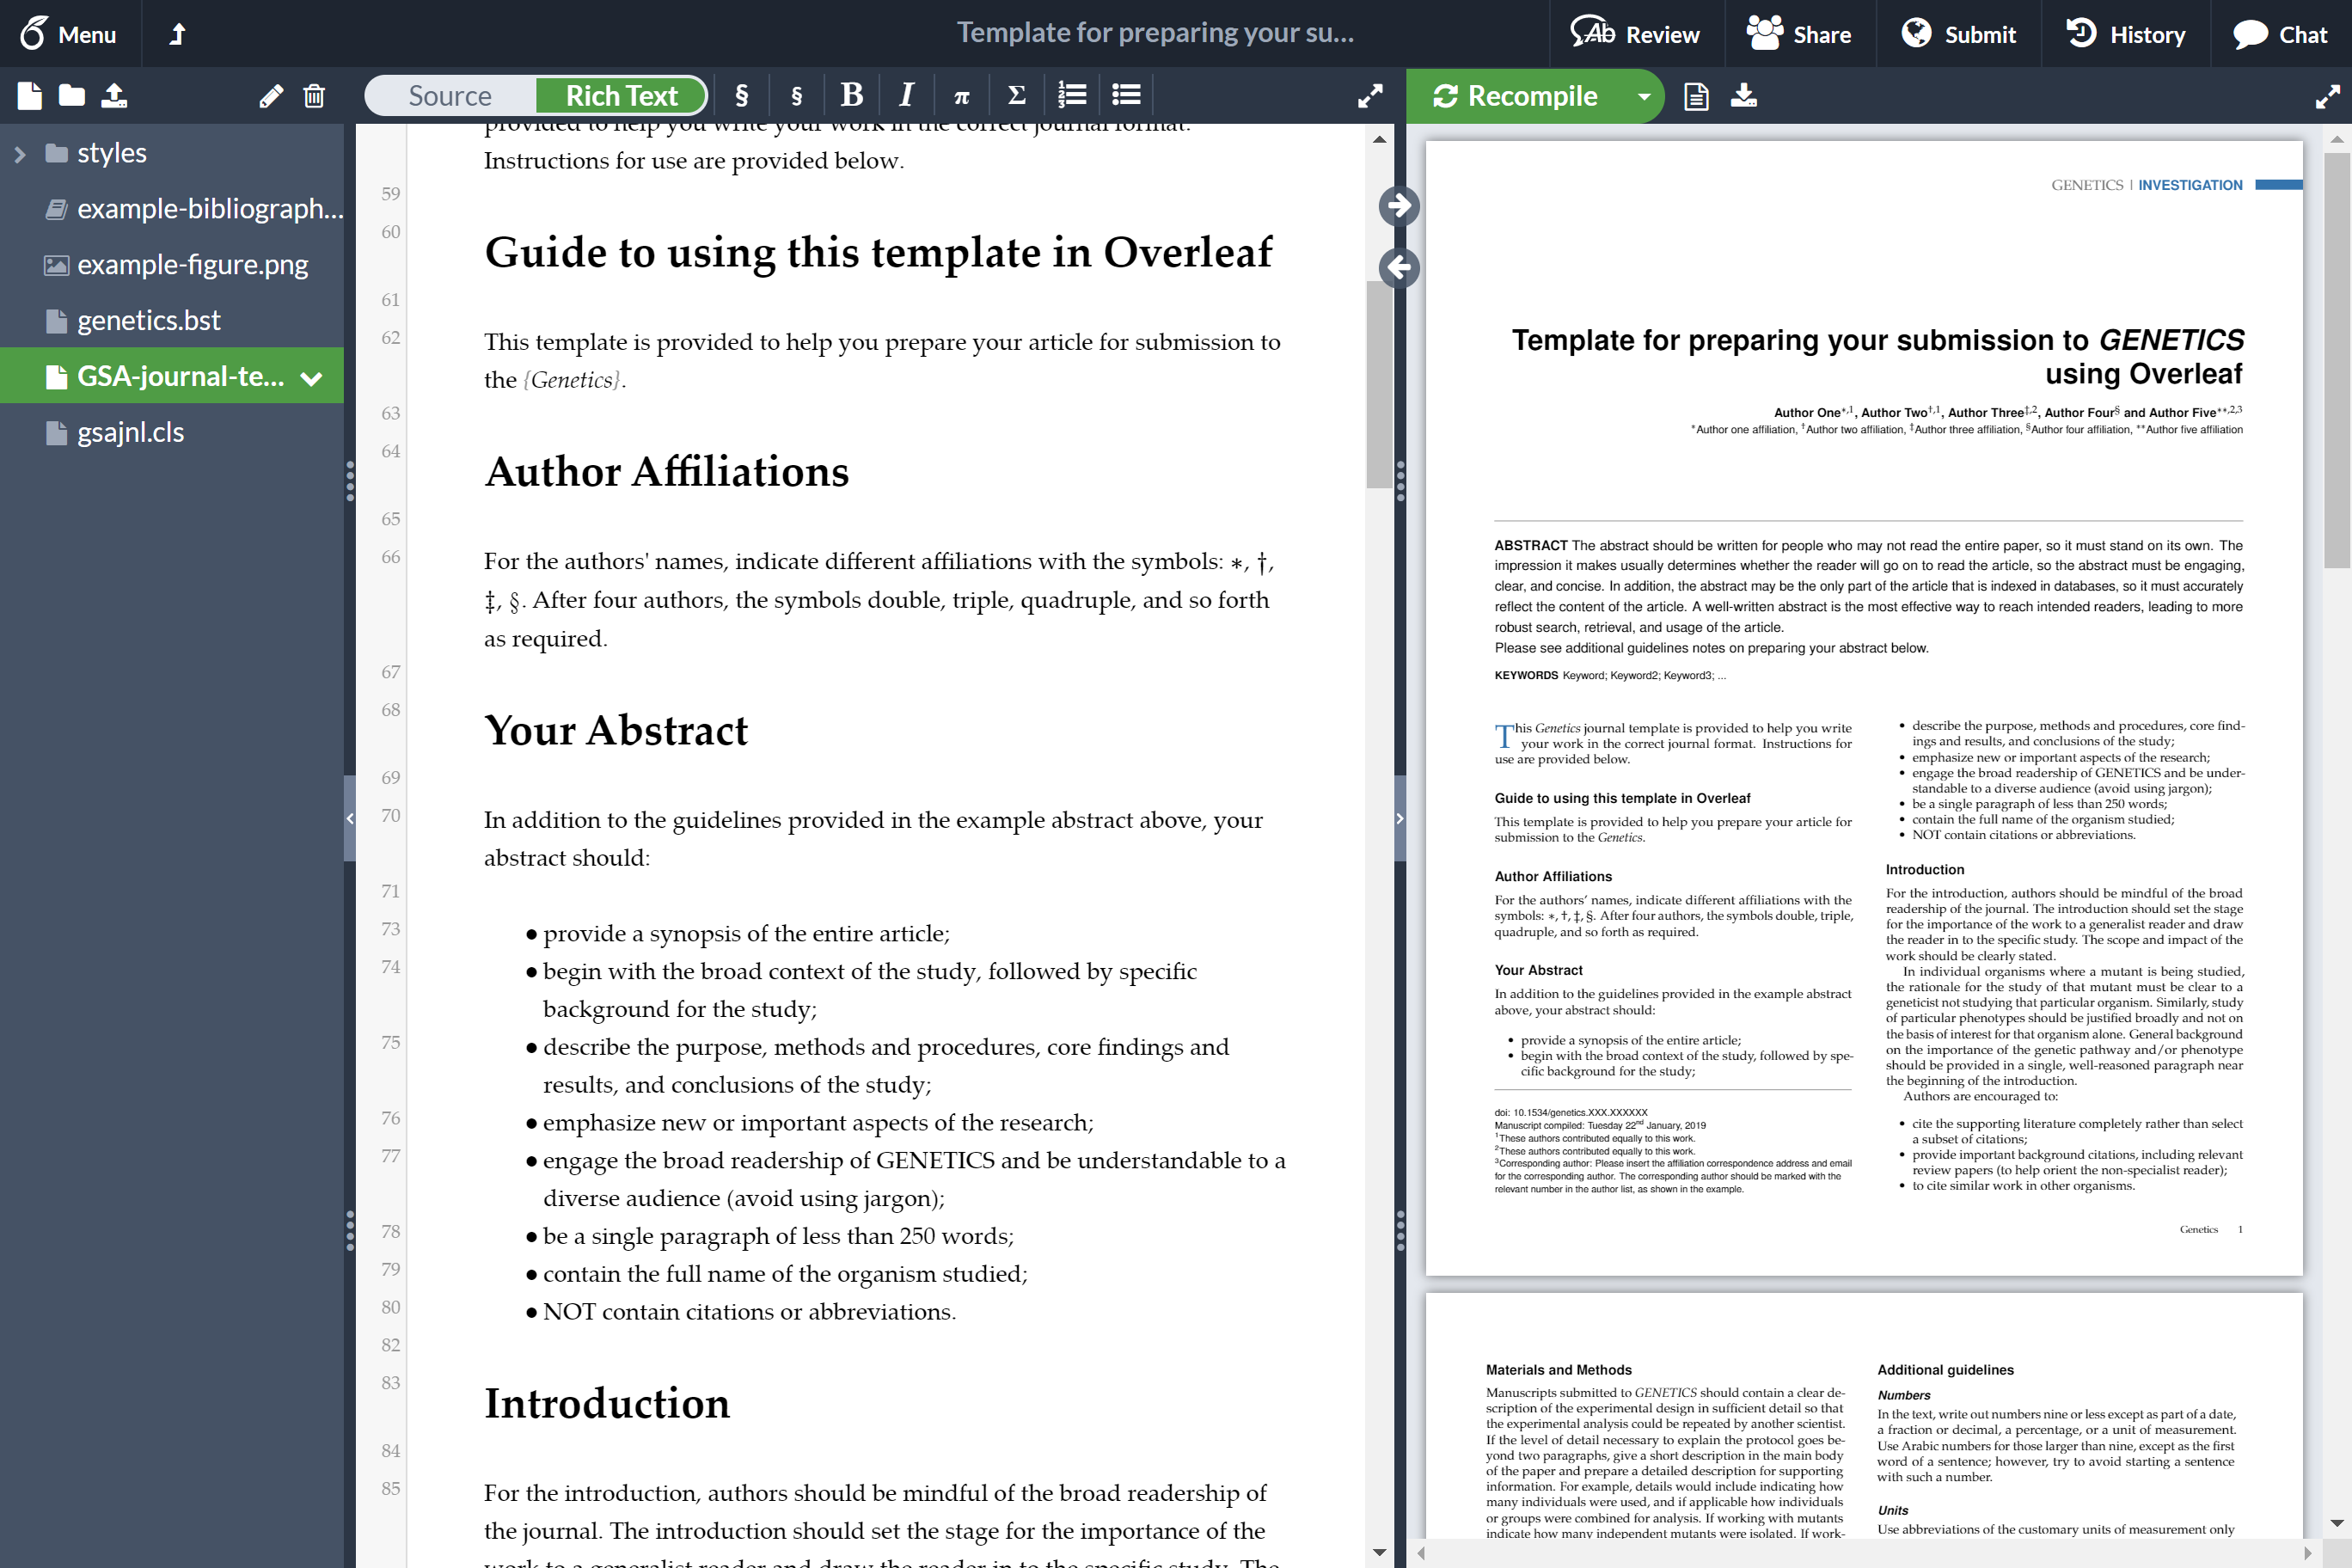
\includegraphics[width=\textwidth]{Lecture1/Figures/Overleaf-journal-template-richtext-example-hires.png}
	\end{center}
\end{frame}


\begin{frame}
	\frametitle{Online distribuce \hologo{LaTeX}u -- sledování změn}
	\begin{center}
		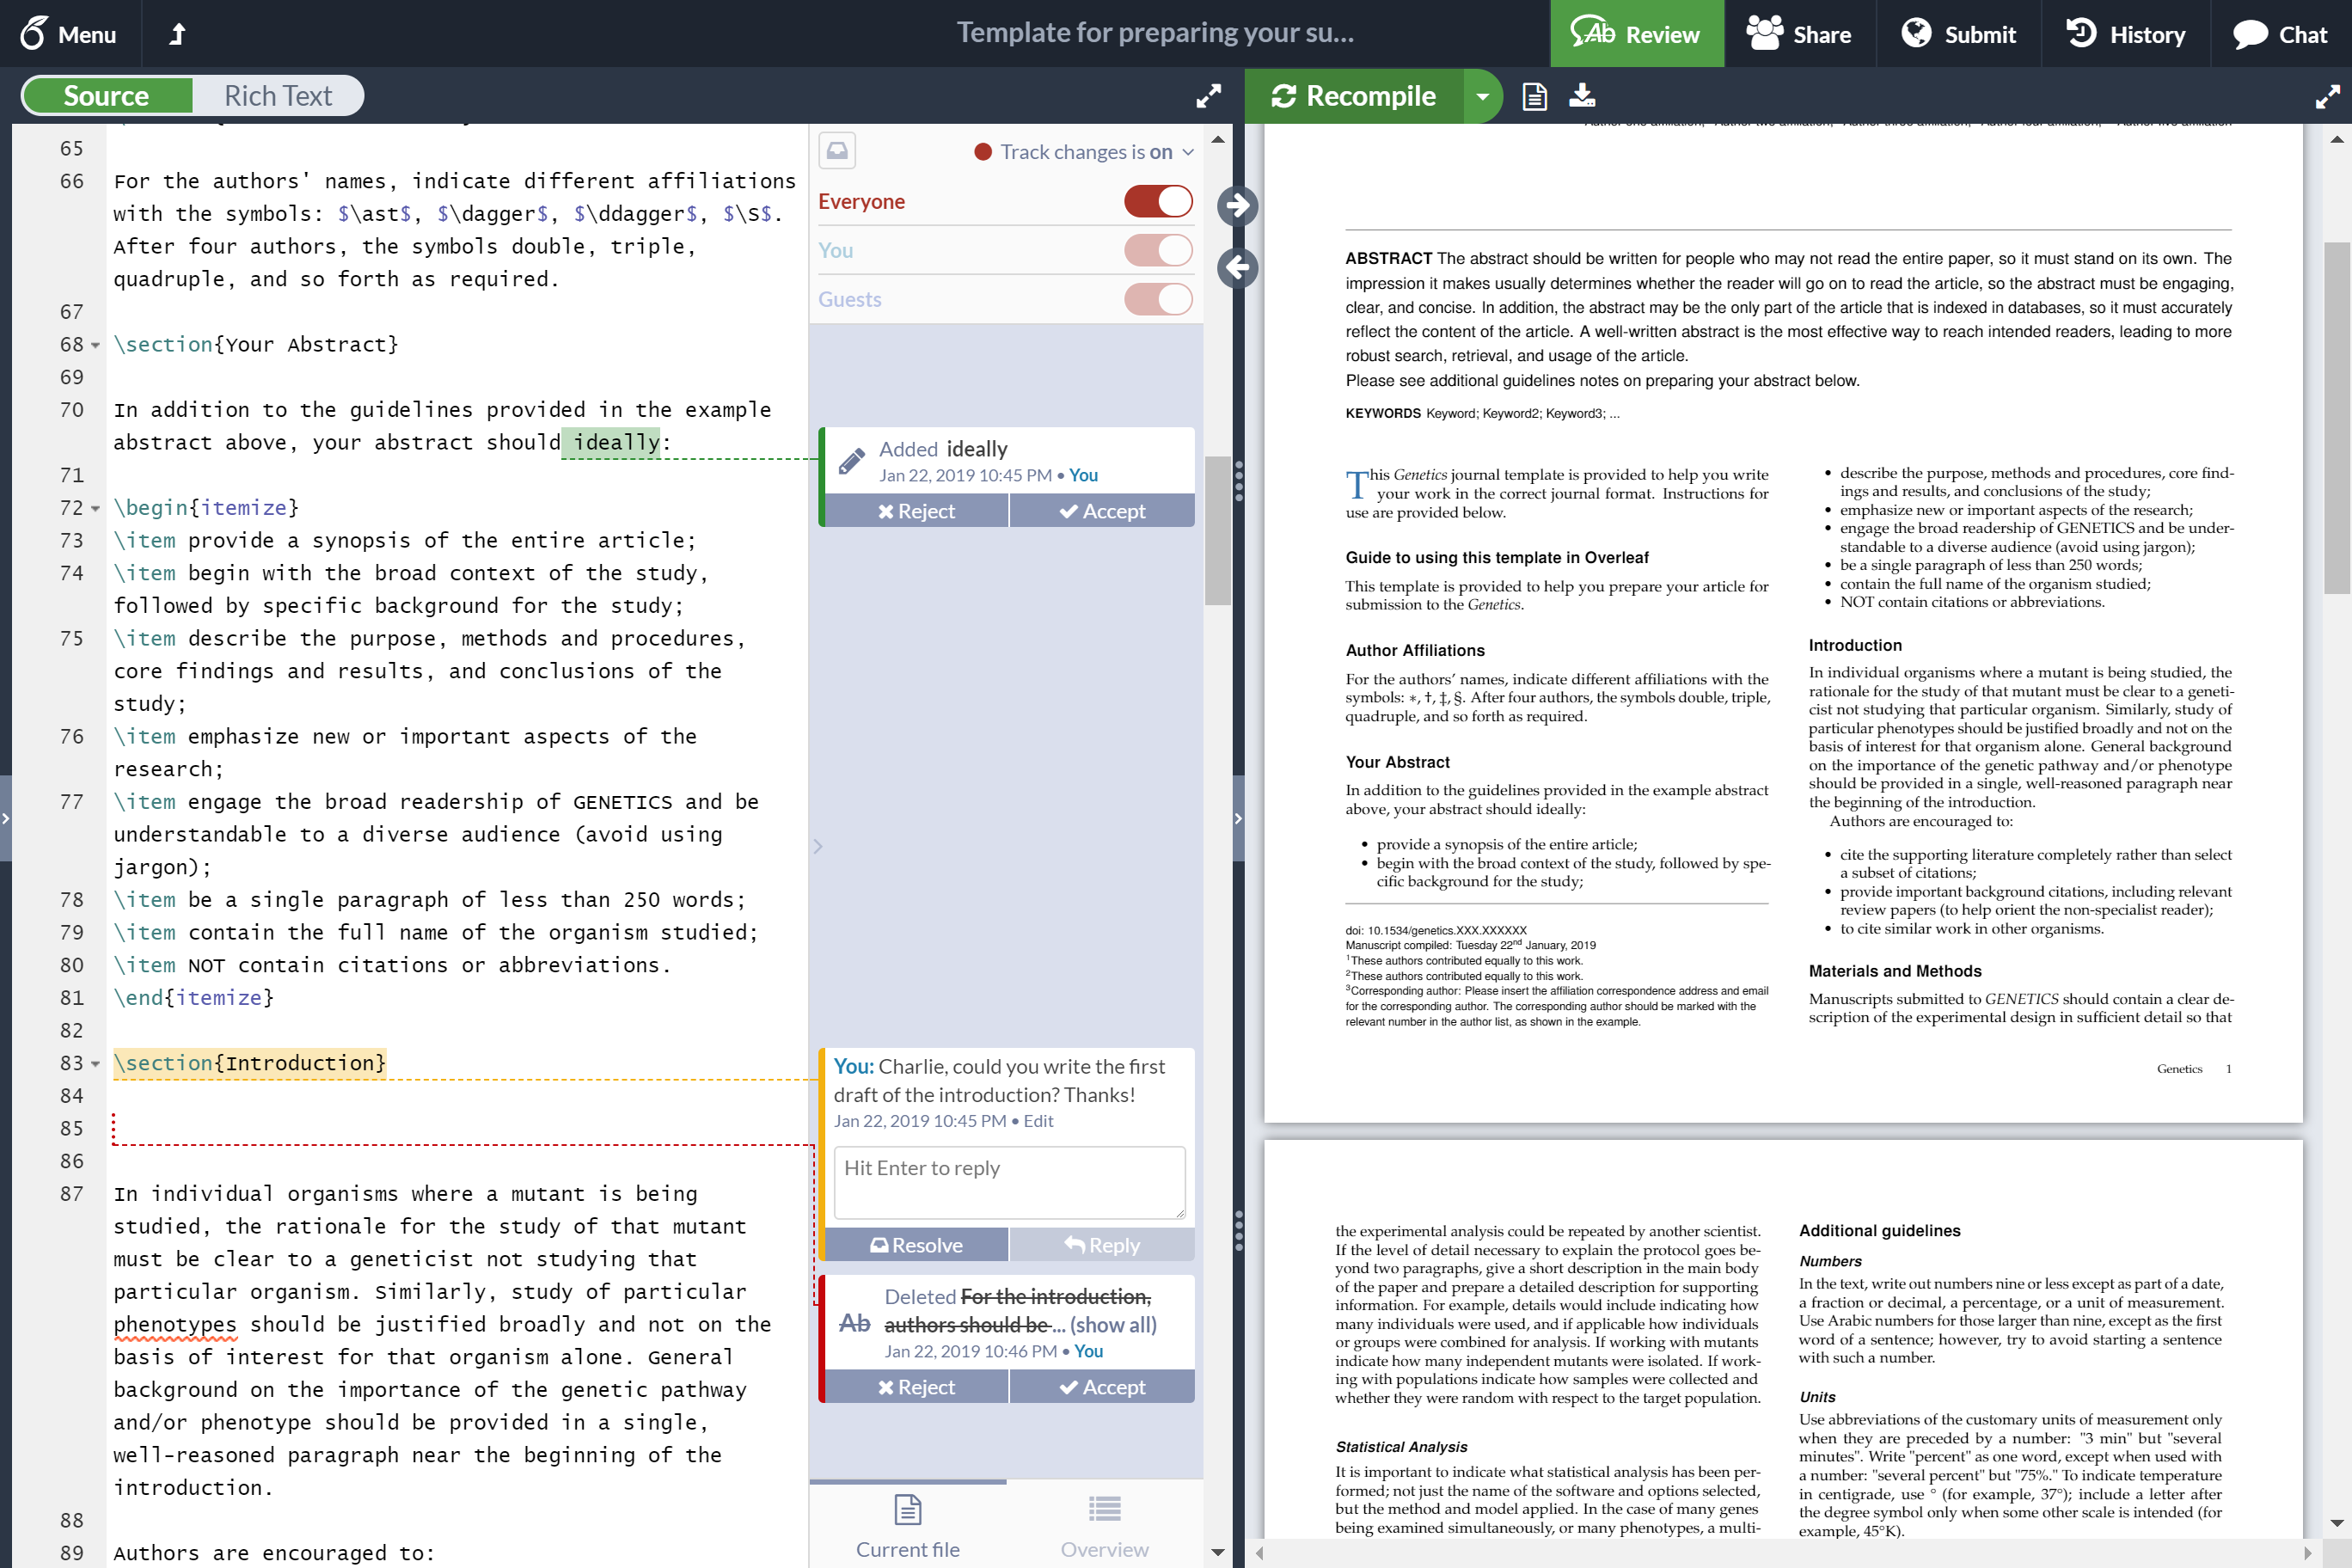
\includegraphics[width=\textwidth]{Lecture1/Figures/Overleaf-journal-template-source-trackchanges-example-hires.png}
	\end{center}
\end{frame}


\begin{frame}
	\frametitle{Overleaf.com -- signalizace chyb při překladu}
	\begin{itemize}
		\item Překladač Overleaf pracuje v tzv.\ \enquote{nonstop} režimu.
		\item Pokud to jen trochu jde, chyby se snaží ignorovat a vysázet dokument za každou cenu. Takový zdrojový kód ale nemusí být bez problémů přeložitelný na jiných systémech.
		\item \alert{Je proto nutné sledovat, zda překlad proběhl bez chyby!}
	\end{itemize}
	\begin{columns}
		\begin{column}{0.45\textwidth}
			\begin{alertblock}{Překlad s chybami}
				\centering
				
\includegraphics[width=0.95\textwidth]{Lecture1/Figures/Overleaf-errors.png}
			\end{alertblock}
		\end{column}
		\begin{column}{0.45\textwidth}
			\begin{block}{Překlad bez chyb}
				\centering
				
\includegraphics[width=0.95\textwidth]{Lecture1/Figures/Overleaf-no-errors.png}
			\end{block}
		\end{column}
	\end{columns}
\end{frame}


\subsection{Editory pro \hologo{LaTeX}}
\begin{frame}
	\frametitle{Editory pro \hologo{LaTeX}}
	\ParagraphCaption{Integrovaná prostředí (IDE)}
	\begin{description}
		\item[Texmaker] -- \url{http://www.xm1math.net/texmaker}
		\item[TeXstudio] -- \url{http://texstudio.sourceforge.net}
		\item[TeXnicCenter] -- \url{https://www.texniccenter.org/}\par{}(v současné době již zastaralé)
	\end{description}
	\ParagraphCaption{Programátorské editory}\par
	Obecně lze použít jakýkoliv programátorský editor - záleží na uživatelově vkusu a zvyku\ldots
	\begin{description}
		\item[Sublime Text] -- \url{http://www.sublimetext.com}
		\item[PSPad]\url{http://www.pspad.com/cz}
	\end{description}
\end{frame}


\subsection{Výstupní formáty a kompilátory}
\begin{frame}
	\frametitle{Výstupní formáty a kompilátory}
	\centering
	\resizebox{\textwidth}{!}{\begin{tikzpicture}
	[
		node/.style = {draw, thick, rectangle, rounded corners, minimum width = 20mm, minimum height = 10mm, align = center},
		file/.style = {draw, thick, rectangle, rounded corners, minimum width = 20mm, minimum height = 10mm, align = center, color = blue!90!black},
		printview/.style = {draw, thick, rectangle, rounded corners, minimum width = 20mm, minimum height = 10mm, align = center, color = green!60!black},
		arrow/.style = {thick, ->, >=stealth},
		fileprocessing/.style = {arrow, color = CornellRed},
		view/.style = {arrow, color = green!60!black},
		node distance = 20mm
	]
	\matrix[row sep = 10mm,column sep = 10mm]
	{
		& \node (DVIFile) [file] {DVI soubor}; & \node (PostscriptFile) [file] {Postscript\\ soubor}; & \\
		\node (LaTeXSourceCode) [file] {zdrojový kód\\ dokumentu}; & & & \node (Print) [printview] {prohlížeč\\ tiskárna};\\
		& \node (PDFFile) [file] {PDF soubor}; & & \\
	};
	\coordinate (Corner1) at (LaTeXSourceCode.south |- DVIFile.west);
	\coordinate (Corner2) at (LaTeXSourceCode.south |- PDFFile.west);
	\draw [fileprocessing] (LaTeXSourceCode.north) -- (Corner1) -- (DVIFile);
	\draw [fileprocessing] (LaTeXSourceCode.south) -- (Corner2) -- (PDFFile);
	\node [CornellRed, below] at (Corner2) {\hologo{pdfLaTeX}};
	\node [CornellRed, above] at (Corner1) {\hologo{LaTeX}};
	\draw (DVIFile) edge [fileprocessing, above] node {dvips} (PostscriptFile);
	\draw (DVIFile) edge [fileprocessing, sloped, below] node {dvipdfmx} (PDFFile);
	\draw [view] (DVIFile) -- (Print.west);
	\draw [view] (PostscriptFile) -| (Print.north);
	\draw (PostscriptFile) edge [fileprocessing, sloped, below] node {ps2pdf} (PDFFile);
	\draw [view] (PDFFile.east) -| (Print.south);
\end{tikzpicture}
\endinput}
\end{frame}


\subsection{Proces kompilace}
\begin{frame}
	\frametitle{Proces kompilace}
	\centering
	\begin{tikzpicture}
	[
		file/.style = {semithick, rounded corners},
		arrow/.style = {semithick, ->, >=stealth},
		doublearrow/.style = {semithick, <->, >=stealth}
	]
	\newcommand{\CellSize}{3}
	\coordinate (SizeX) at (\CellSize, 0);
	\coordinate (SizeY) at (0, \CellSize);
	\coordinate (FileBoxSize) at ($4*(SizeX) + 2*(SizeY)$);
	\coordinate (FileBoxLabelOffset) at ($2*(SizeX) + 1*(SizeY)$);

	\coordinate (DocSource) at ($0*(SizeX) + 11*(SizeY)$);
	\coordinate (LaTeXImpl) at ($0*(SizeX) + 8*(SizeY)$);
	\coordinate (Packages) at ($0*(SizeX) + 5*(SizeY)$);

	\coordinate (PdfFile) at ($24*(SizeX) + 11*(SizeY)$);
	\coordinate (LogFile) at ($24*(SizeX) + 5*(SizeY)$);

	\coordinate (ToCFile) at ($3*(SizeX) + 18*(SizeY)$);
	\coordinate (LoTFile) at ($9*(SizeX) + 18*(SizeY)$);
	\coordinate (LoFFile) at ($15*(SizeX) + 18*(SizeY)$);
	\coordinate (AuxFile) at ($21*(SizeX) + 18*(SizeY)$);

	\coordinate (TeXCompiler) at ($10*(SizeX) + 6*(SizeY)$);

	\coordinate (DocumentIndex) at ($19*(SizeX) + 1*(SizeY)$);
	\coordinate (Bibliography) at ($9*(SizeX) + 1*(SizeY)$);

%	\draw [step=\CellSize, lightgray] (0, 0) grid ++($33*(SizeX) + 21*(SizeY)$);

	\fill [file, color = green!60!black] (DocSource) rectangle ++(FileBoxSize);
	\node [font = \large] at ($(DocSource) + (FileBoxLabelOffset)$) {a.tex};

	\draw [file] (LaTeXImpl) rectangle ++(FileBoxSize);
	\node at ($(LaTeXImpl) + (FileBoxLabelOffset)$) {\hologo{LaTeX}};

	\draw [file] (Packages) rectangle ++(FileBoxSize);
	\node at ($(Packages) + (FileBoxLabelOffset)$) {Balíky};

	\fill [file, color = green!60!black] (PdfFile) rectangle ++(FileBoxSize);
	\node at ($(PdfFile) + (FileBoxLabelOffset)$) {a.pdf};

	\draw [file] (LogFile) rectangle ++(FileBoxSize);
	\node at ($(LogFile) + (FileBoxLabelOffset)$) {a.log};

	\draw [file] (ToCFile) rectangle ++(FileBoxSize);
	\node at ($(ToCFile) + (FileBoxLabelOffset)$) {a.toc};

	\draw [file] (LoTFile) rectangle ++(FileBoxSize);
	\node at ($(LoTFile) + (FileBoxLabelOffset)$) {a.lot};

	\draw [file] (LoFFile) rectangle ++(FileBoxSize);
	\node at ($(LoFFile) + (FileBoxLabelOffset)$) {a.lof};

	\draw [file] (AuxFile) rectangle ++(FileBoxSize);
	\node at ($(AuxFile) + (FileBoxLabelOffset)$) {a.aux};

	\fill [thick, fill = lightgray, rounded corners] (TeXCompiler) rectangle ++($8*(SizeX) + 6*(SizeY)$);
	\node [font = \Large] at ($(TeXCompiler) + 4*(SizeX) + 3*(SizeY)$) {\hologo{pdfLaTeX}};

	\draw [arrow] ($(DocSource) + 4*(SizeX) + 1*(SizeY)$) -- ($(TeXCompiler) + 4*(SizeY)$);
	\draw [arrow] ($(LaTeXImpl) + 4*(SizeX) + 1*(SizeY)$) -- ($(TeXCompiler) + 3*(SizeY)$);
	\draw [arrow] ($(Packages) + 4*(SizeX) + 1*(SizeY)$) -- ($(TeXCompiler) + 2*(SizeY)$);

	\draw [arrow] ($(TeXCompiler) + 8*(SizeX) + 4*(SizeY)$) -- ($(PdfFile) + 0*(SizeX) + 1*(SizeY)$);
	\draw [arrow] ($(TeXCompiler) + 8*(SizeX) + 2*(SizeY)$) -- ($(LogFile) + 0*(SizeX) + 1*(SizeY)$);

	\draw ($(ToCFile) + 1.5*(SizeX)$) edge [arrow] node [pos = 0.4, sloped, below, color = CornellRed, font = \tiny\ttfamily] {\textbackslash{}tableofcontents} ($(TeXCompiler) + 0*(SizeX) + 5.5*(SizeY)$);

	\draw ($(TeXCompiler) + 0.5*(SizeX) + 6*(SizeY)$) edge [arrow] node [midway, sloped, above, color = CornellRed, font = \tiny\ttfamily] {\textbackslash{}section,\ldots} ($(ToCFile) + 2.5*(SizeX)$);

	\draw ($(LoTFile) + 1.5*(SizeX)$) edge [arrow] node [midway, sloped, below, color = CornellRed, font = \tiny\ttfamily] {\textbackslash{}listoftables} ($(TeXCompiler) + 2*(SizeX) + 6*(SizeY)$);

	\draw ($(TeXCompiler) + 3*(SizeX) + 6*(SizeY)$) edge [arrow] node [midway, sloped, above, color = CornellRed, font = \tiny\ttfamily] {\textbackslash{}caption} ($(LoTFile) + 2.5*(SizeX)$);

	\draw ($(TeXCompiler) + 6*(SizeX) + 6*(SizeY)$) edge [arrow] node [midway, sloped, below, color = CornellRed, font = \tiny\ttfamily] {\textbackslash{}caption} ($(LoFFile) + 2.5*(SizeX)$);

	\draw ($(LoFFile) + 1.5*(SizeX)$) edge [arrow] node [midway, sloped, above, color = CornellRed, font = \tiny\ttfamily] {\textbackslash{}listoffigures} ($(TeXCompiler) + 5*(SizeX) + 6*(SizeY)$);


	\draw ($(TeXCompiler) + 7.5*(SizeX) + 6*(SizeY)$) edge [arrow] node [midway, sloped, above, color = CornellRed, font = \tiny\ttfamily] {\textbackslash{}label} ($(AuxFile) + 1.5*(SizeX)$);

	\draw ($(AuxFile) + 2.5*(SizeX)$) edge [arrow] node [midway, sloped, below, color = CornellRed, font = \tiny\ttfamily] {\textbackslash{}ref} ($(TeXCompiler) + 8*(SizeX) + 5.5*(SizeY)$);

	\node [draw, thick, cloud, aspect = 2.75] at (Bibliography) (BibliographyNode) {Literatura};
	\node [draw, thick, cloud, aspect = 2] at (DocumentIndex) (DocumentIndexNode) {Rejstřík};

	\draw [doublearrow] ($(TeXCompiler) + 2*(SizeX)$) -- (BibliographyNode.north);
	\draw [doublearrow] ($(TeXCompiler) + 6*(SizeX)$) -- (DocumentIndexNode.north);
\end{tikzpicture}
\endinput

\end{frame}


\begin{frame}
	\frametitle{Ukázky sazby -- úmluva}
	\begin{itemize}
		\item Předchozí ukázka sazby dokumentu i tato prezentace vznikla za použití \hologo{LaTeX}u.
		\item Je však jasné, že sazba dokumentu na stranu formátu A4 a~sazba prezentace se řídí jinými parametry -- rozměry stránky, použitý font a~jeho velikost, barvy a tak dále.
		\item Pokud nebude výsledek sazby daného typografického prvku v prezentaci a \enquote{papírovém dokumentu} diametrálně odlišný, bude sazba demonstrována přímo v prezentaci. Ve svém dokumentu však uvidíte sice stejný prvek, ale vysázený pravděpodobně jiným fontem, v jiné barvě a tak dále.
	\end{itemize}
\end{frame}


\begin{frame}[allowframebreaks,fragile]
	\frametitle{Ukázky sazby -- nastavení}
	Ukázky sazby \enquote{papírového dokumentu} probíhají vždy s~následujícím nastavením:\par
	\begin{BVerbatim}
\documentclass[10pt, a4paper]{article}
\usepackage{cmap}
\usepackage[utf8]{inputenc}
\usepackage[T1]{fontenc}
\usepackage{lmodern}
\usepackage[czech]{babel}
\begin{document}
...
\end{document}
	\end{BVerbatim}
	\par
	 Dále mohou být vloženy aktuálně demonstrované balíky maker.\par
	 Překlad probíhá pomocí \hologo{pdfLaTeX}u.
\end{frame}

\endinput
